\documentclass[a4paper,12pt]{article}
\usepackage[utf8]{inputenc}
\usepackage{graphicx}
\usepackage{multicolumn}
\usepackage{multirow}
\usepackage{booktabs}
\usepackage[indent=0pt,skip=3mm]{parskip}
\usepackage{array}
\usepackage{commath} % for abs ||
\usepackage{listings}             % Include the listings-package
\usepackage{tabs}
\usepackage{mathtools}
% \usepackage{colortbl}
% \usepackage{url}
\usepackage{hyperref}
\usepackage{datetime}
\usepackage[ top=5cm, left=1.5cm, right=1.5cm, headheight=4cm,bottom=1cm]{geometry}
\usepackage{lastpage} % include last page numbering
\usepackage{fancyhdr}
\usepackage[table]{xcolor}% ctan.org/pkg/xcolor %FOR COLORS
% \usepackage{frame}
\settimeformat{xxivtime}
\setdefaultdate{\ddmmyyyydate}
\hyphenation{matriz}
\graphicspath{{figures/}{./images/}}
\newcommand{\eq}[1]{$#1$}
\newcommand{\head}[1]{{\bfseries #1}}
\newcommand{\header}[2][\tiny]{{\bfseries #1 #2}}
\newcommand{\mysubject}[1]{Metodos para encontrar raíces.\\}
%%%%%%%%%%%%%%%%%%%%%%%%%%%%%%%%%%%%%%%%%%%%%%%%%%%%%%%%%%%%%%%%%%%%%%
%%%%%%%%%%%%%%%%%%%%%%%%%%%%%%%%%%%%%%%%%
\newsavebox{\mytabularheader}
\newsavebox{\mytabularheadertitle}
\setlength{\extrarowheight}{0.1cm}
%----------------------------------------------------------------------------------
%-----------------------------------------------------------------------------------------------
\sbox{\mytabularheadertitle}{%
  \begin{minipage}{.52\textwidth}
    \begin{center}
        \bfseries \scriptsize  UNIVERSIDAD NACIONAL DE SAN AGUSTIN\\
        FACULTAD DE INGENIERÍA DE PRODUCCIÓN Y SERVICIOS\\
        ESCUELA PROFESIONAL DE INGENIERÍA DE SISTEMA\\[3mm]
    \end{center}
  \end{minipage}
}

\sbox{\mytabularheader}{%
    \begin{minipage}{\textwidth}
        \centering
        \begin{tabular}{cp{8cm}c}
            
\includegraphics[scale=0.3]{epis_logo.png} & 
            \usebox{\mytabularheadertitle} &
            
\includegraphics[scale=0.04]{abet_logo.png} \\
            % \hline
            \multicolumn{3}{c}{Formato: Guía de Práctica de Laboratorio / Talleres / Centros de Simulación}\\
             &\multicolumn{1}{c}{Aprobación:  2022/03/01 Código: GUIA-PRLE-001} &  \\
        \end{tabular}
    \end{minipage}
}
%---------------------------------------
\renewcommand{\headrulewidth}{0pt}
\fancypagestyle{plain}{%
  \fancyhf{}%
  \fancyhf[ch]{\usebox{\mytabularheader}}
}
%--------------------------------------
\pagestyle{plain}
%%%%%%%%%%%%%%%%%%%%%%%%%%%%%%%%%%%%%%%%%%%%%%%%%%%%%%%%%%%%%%%%%%%%%%%%%%%%%%%%%%%%%%%%%%
\definecolor{blackRed}{cmyk}{0,81,76,31}

\begin{document}    
\lstset{language=Python,frame=single, firstnumber=1,basicstyle=\footnotesize,
numbers=left,showspaces=false,showstringspaces=false}   
    \begin{table}[t]
        \centering
        \begin{tabular}{|p{2.3cm}<{:}|m{1.7cm}|m{2.4cm}|m{2cm}|m{3cm}|m{0.6cm}|}
            \multicolumn{6}{c}{\cellcolor{blackRed}{\leavevmode\color{white}\header{INFORMACIÓN BÁSICA}}}\\
            \hline
            \header{ASIGNATURA} & \multicolumn{5}{c}{\header[\footnotesize]{Física Computacional.}}\\
            \hline
            \header{\mbox{TÍTULO DE LA} PRÁCTICA} & \multicolumn{5}{c}{\header[\footnotesize]{Metodos para encontrar raíces.}}\\
            \hline
            \header{\mbox{NÚMERO DE} PRÁCTICA} & {\header[\footnotesize]{09}} & \header{AÑO LECTIVO:} & {\header[\footnotesize]{2022-A}} & \header{NRO. SEMESTRE:} & \header[\footnotesize]{VII}\\
            \hline
            \header{\mbox{FECHA DE} \mbox{PRESENTACIÓN}} & \header{\today} & \header{HORA DE \mbox{PRESENTACIÓN:}} & \multicolumn{3}{c}{\header[\footnotesize]{\currenttime}}\\
            \hline
            \multicolumn{4}{l}{\header[\footnotesize]{Integrante(s): Alván Ventura Edsel Yael}} & \header{NOTA} & \\
            \hline
            \multicolumn{6}{l}{\header[\footnotesize]{DOCENTE(s):} \header[\footnotesize]{Danny Giancarlo Apaza Veliz.}} \\  
            \bottomrule
        \end{tabular}
    \end{table}
    \title{Práctica 9\\\mysubject\\Física Computacional}
    \date{\vspace{-5ex}}
    \maketitle
    \begin{center}
        Escrito por\\
        Alván Ventura, Edsel Yael\\ \texttt{ealvan@unsa.edu.pe}
        \\[3mm]
        Profesor\\Apaza Veliz, Danny Giancarlo\\ \texttt{dapazav@unsa.edu.pe}\\[3mm]
        \today
    \end{center}
    % \newgeometry{top=2cm}
    \enlargethispage{\baselineskip}
    % \newpage
    Aplicando los métodos de resolución para ecuaciones no lineales resuelva
    las siguientes ecuaciones. La elección del método y el lenguaje de programación es libre.

    \section{Análisis}
    El análisis mostrados en las siguientes fotografías son de los métodos Newton Raphson y Secante.
    
    El método Newton Raphson usa la derivada de la función para encontrar la siguiente aproximación a la raíz.
    Viendo que cada vez, se acerca a la raiz verdadera. Pero para usarlo se necesita la derivada de la función, la cual 
    puede ser dificil de hallar en algunos casos. 
    La ecuación del Método Newton Raphson es:
    \begin{equation}
        x_{n+1} = x_n - \frac{f(x_n)}{f'(x_n)}
    \end{equation}
    A continuación se muestra el análisis:
    \begin{figure}[h]
        \centering 
        \includegraphics[width=0.8\textwidth]{method1.jpg}
    \end{figure}

    Mientras que el Método de la Secante, usa las diferencias finitas para aproximar la derivada de la función 
    conforme se avanza a la raiz, es más conveniente usarla cuando es muy dificil de hallar la derivada de una función.
    La idea en sí, es la misma que el Método Newton Raphson, pero la ventaja es que no necesitamos hallar la derivada analíticamente.

    Una desventaja, es que Newton Raphson es más rápido que el Método de la Secante.

    La formula del Método Secante es:
    \begin{equation}
        x_{n+1} = x_n - \frac{f(x_n)*(x_{n} - x_{n-1})}{f(x_n) - f(x_{n-1})}
    \end{equation}
    \newpage
    \begin{figure}[t]
        \centering 
        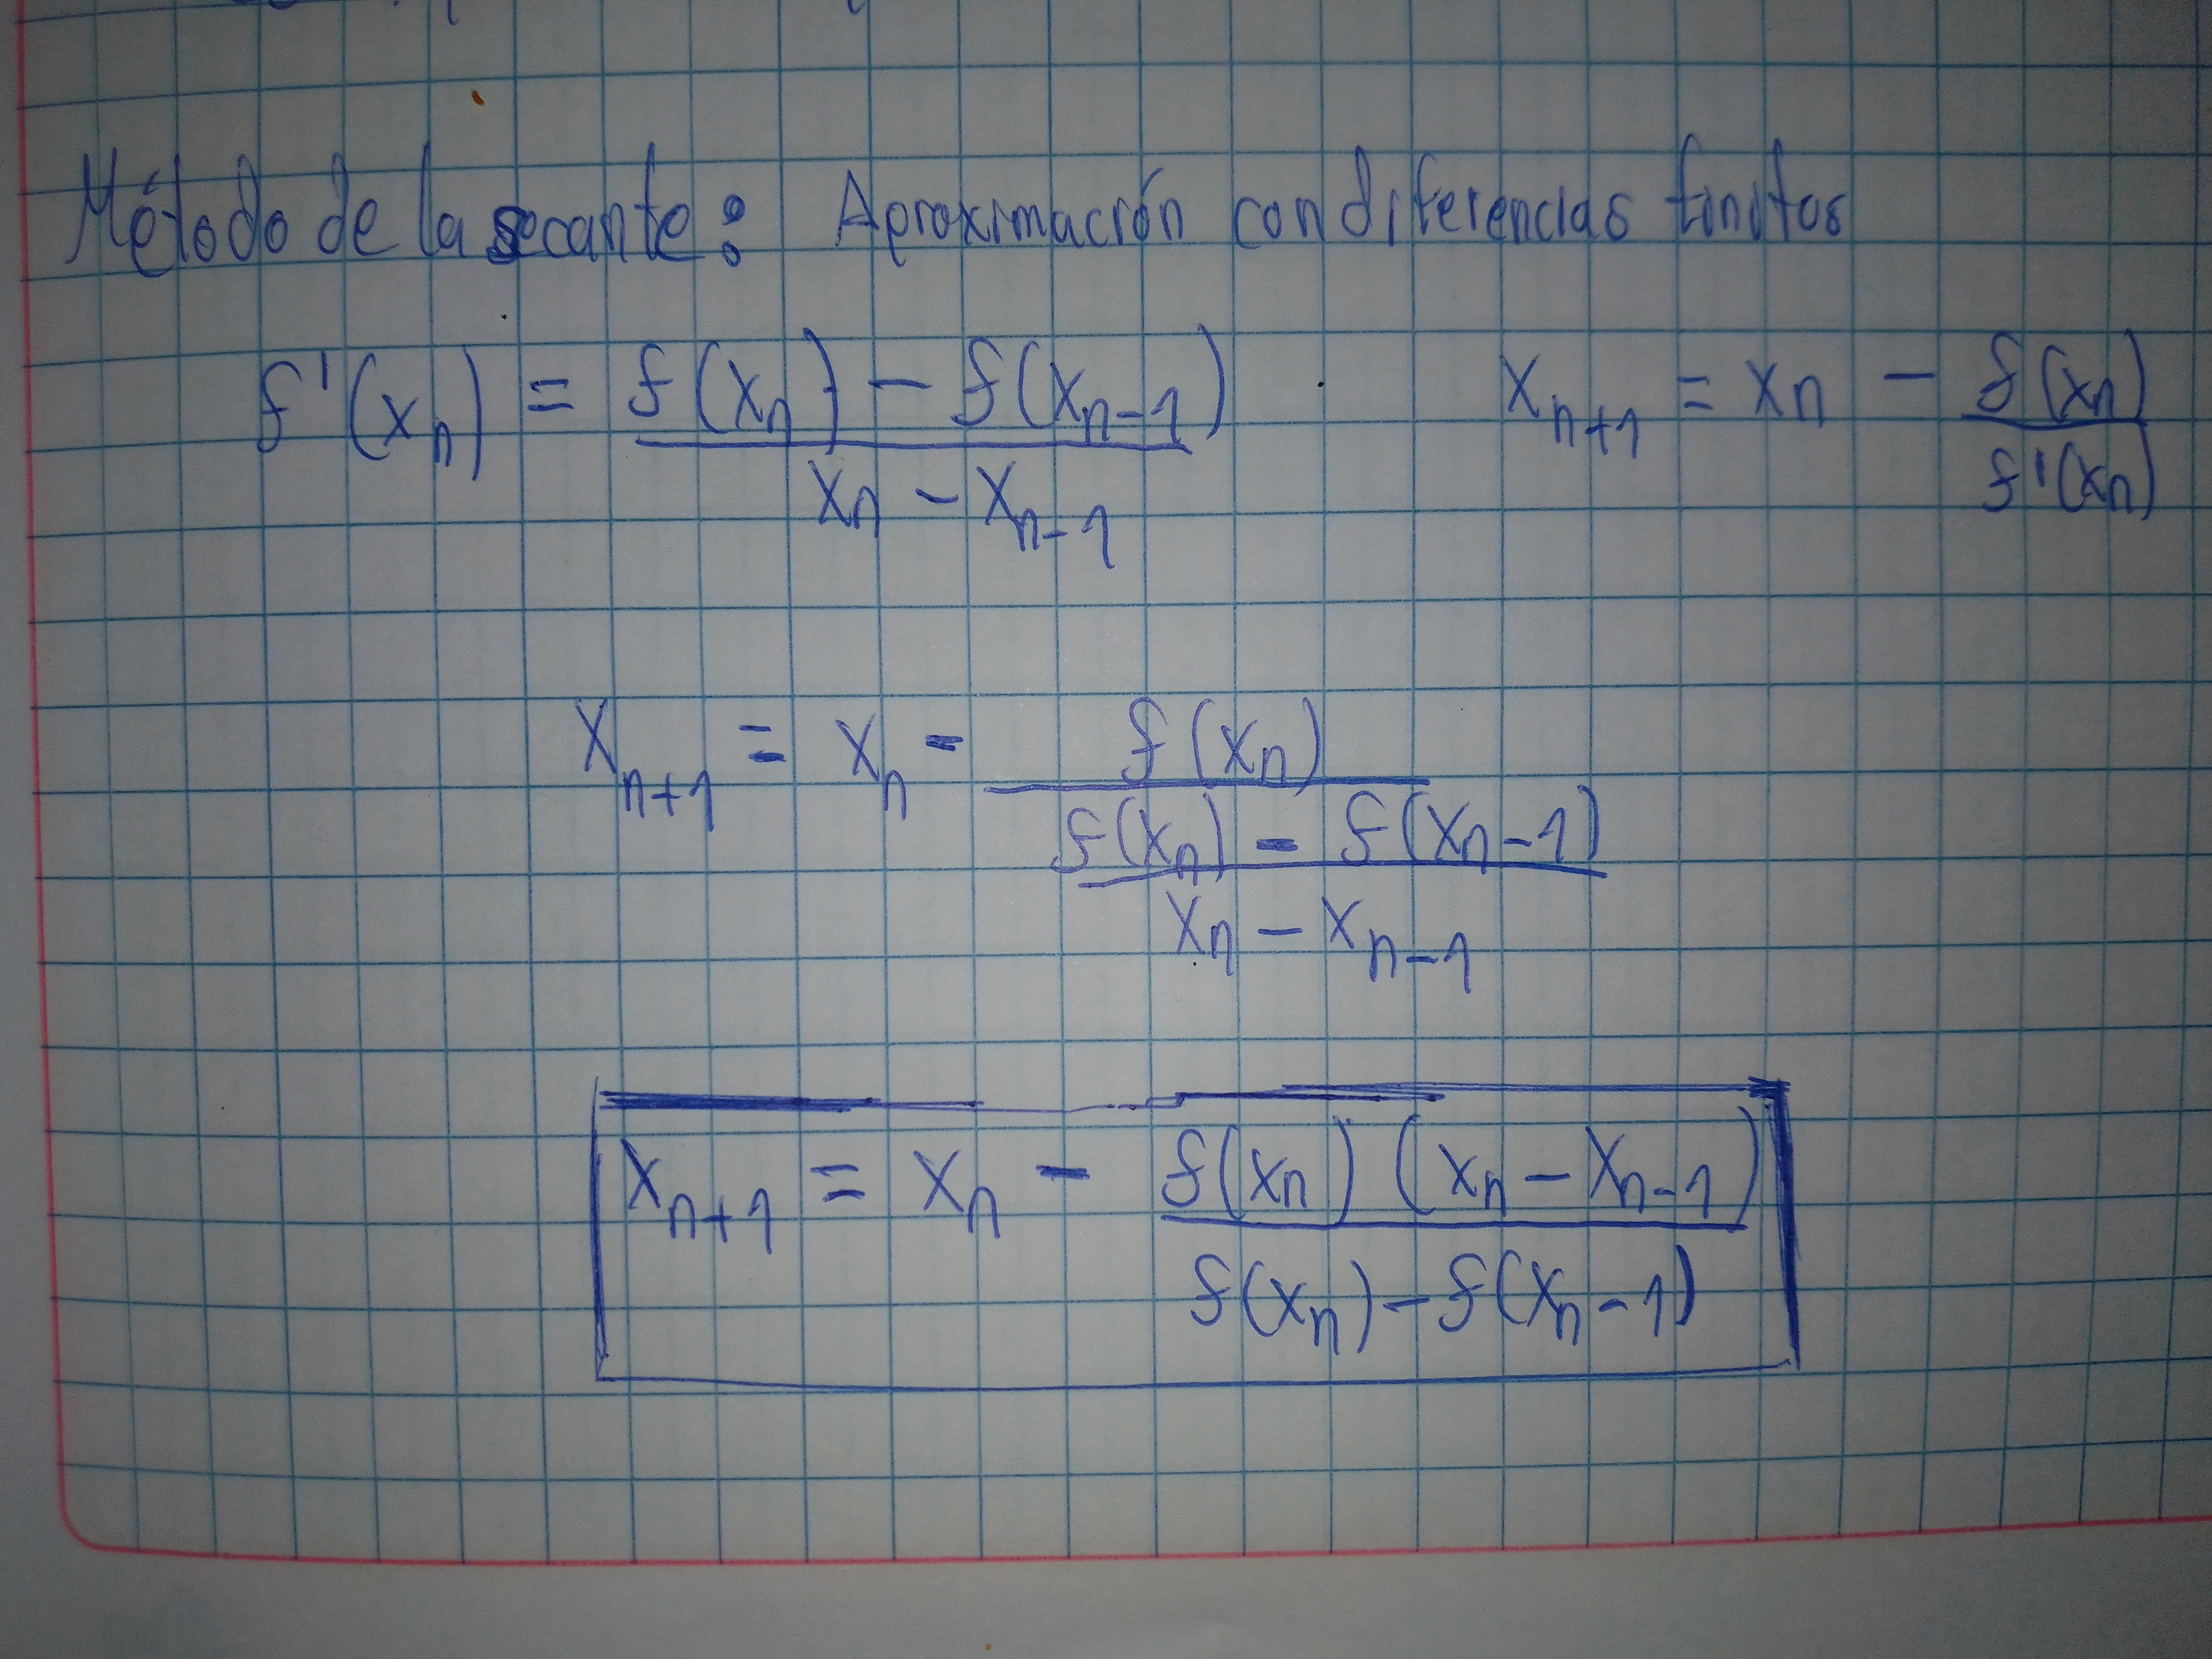
\includegraphics[width=0.8\textwidth]{method2.jpg}
    \end{figure}    
    \section{Implementación}
    A continuación se muestra la implementación del Método de Newton Raphson:
    \lstinputlisting[title=Método Raphson Newton]{newton-rhapson.py}

    A continuación se muestra la implementación del Método de la Secante:
    \lstinputlisting[title=Método Secante]{secante.py}

    \newpage

    \section{Problema 1}
    Calcule:
    \begin{equation}
        y = e^{-x}
    \end{equation}
    
    La gráfica de la función es:

    \begin{figure}[h]
        \centering
        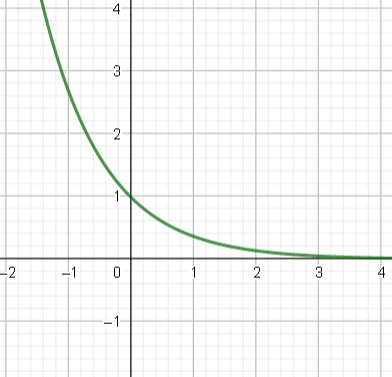
\includegraphics[width=0.4\textwidth]{f1.PNG}
    \end{figure}

    Se decidió usar 
    el Método de Newton Raphson, la razón es que su derivada es fácil 
    de hallar y por lo tanto
    podemos hallar las raíces por este método.

    Pero si suponemos que vamos a usar el punto -3, podemos ver que terminara en 
    que la solución es 0, de acuerdo al Método Newton Raphson.

\begin{lstlisting}
#Funcion f(x)
def f(x):
    fx = lambda x: m.e**(-1*x)
    return fx(x)
#Derivada de la funcion f(x)
def df(x):
    dfx = lambda x: -1*m.e**(-1*x)
    return dfx(x)

if __name__ == "__main__":
    mystr = newtonRaphson(-3)
    print(mystr) #contiene todos las iteraciones
\end{lstlisting}
    \newpage
    El resultado de las iteraciones es:
    \begin{figure}[h]
        \centering
        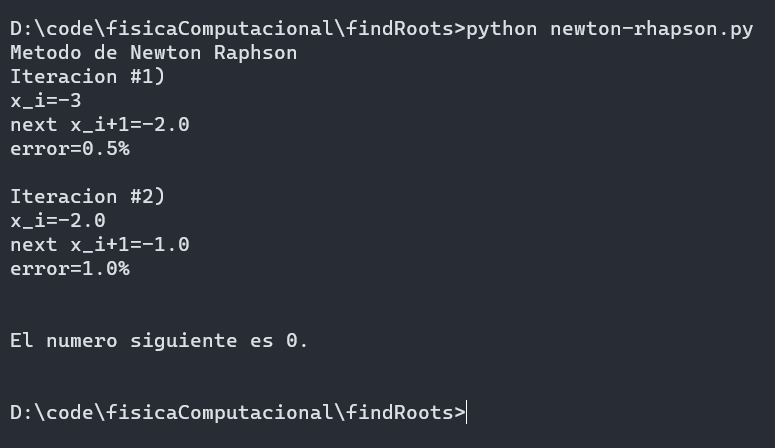
\includegraphics[width=0.5\textwidth]{f1console.PNG}
    \end{figure}

    \section{Problema 2}
    Calcule:
    \begin{equation}
        y = e^x - x        
    \end{equation}

    La gráfica de la función es:
    \begin{figure}[h]
        \centering
        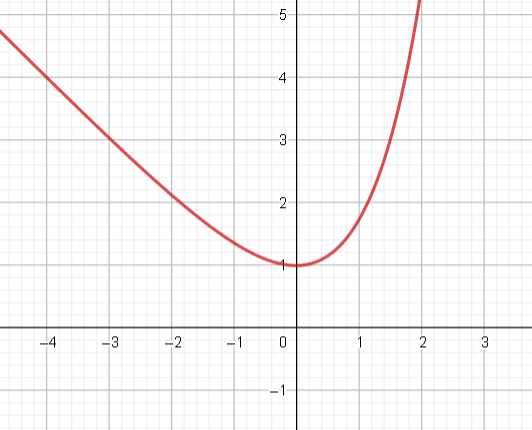
\includegraphics[width=0.4\textwidth]{f2.PNG}
    \end{figure}

    Se decidió usar 
    el Método de Newton Raphson porque su derivada es fácil 
    de hallar y por lo tanto los requisitos que necesita Newton Raphson se han cumplido.

    Pero como suponemos si usamos cualquier punto, podemos ver que terminara en 
    que la solución no la hallará, pues no tiene ninguna intersección con el eje X.
    Asi que irá de un lado hacia a otro en un bucle sin fín, si es que no le decimos explícitamente
    que si el error es mayor que el anterior error, entonces significa que puede repetirse este comportamiento.

\begin{lstlisting}
#condicion para que no sea un bucle infinito
if(bufferr < current_error):
        mystr += f"El error actual({round(current_error,4)}%) es mayor "
        mystr += f"que el anterior({round(bufferr,4)}%)"
        mystr += f"\nSignifica que no se encontro la raiz con el punto {sig}"
        mystr += " \no la ecuacion no tiene raices"
        return mystr
\end{lstlisting}    
En la siguientes funciones iniciales se implementa 
la derivada y la función para la realización del Método Raphson.
\begin{lstlisting}
#Funcion f(x)
def f(x):
    fx = lambda x: m.e**x - x
    return fx(x)
#Derivada de la funcion f(x)
def df(x):
    dfx = lambda x: m.e**x - 1
    return dfx(x)

if __name__ == "__main__":
    mystr = newtonRaphson(4)
    print(mystr) #contiene todos las iteraciones
\end{lstlisting}

    El resultado de las iteraciones es:
    \begin{figure}[h]
        \centering
        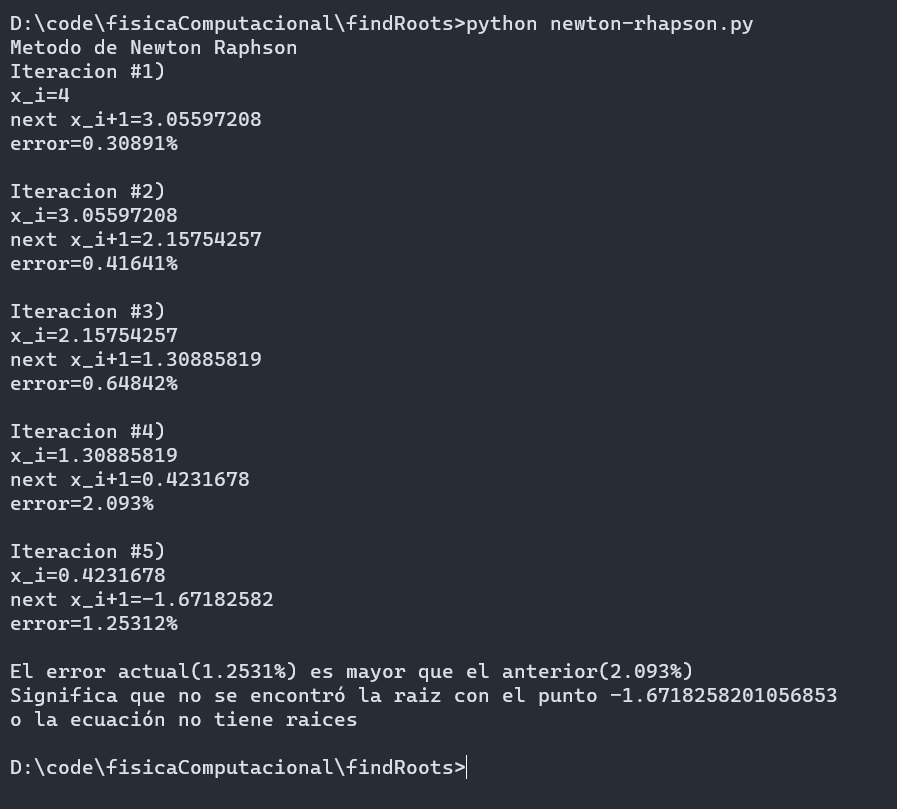
\includegraphics[width=0.5\textwidth]{f2console.PNG}
    \end{figure}
    \newpage
    \section{Problema 3}
    Calcule:
    \begin{equation}
        10e^{\frac{x}{2}}cos(2x)-4
    \end{equation}

    La gráfica de la función es:
    \begin{figure}[h]
        \centering
        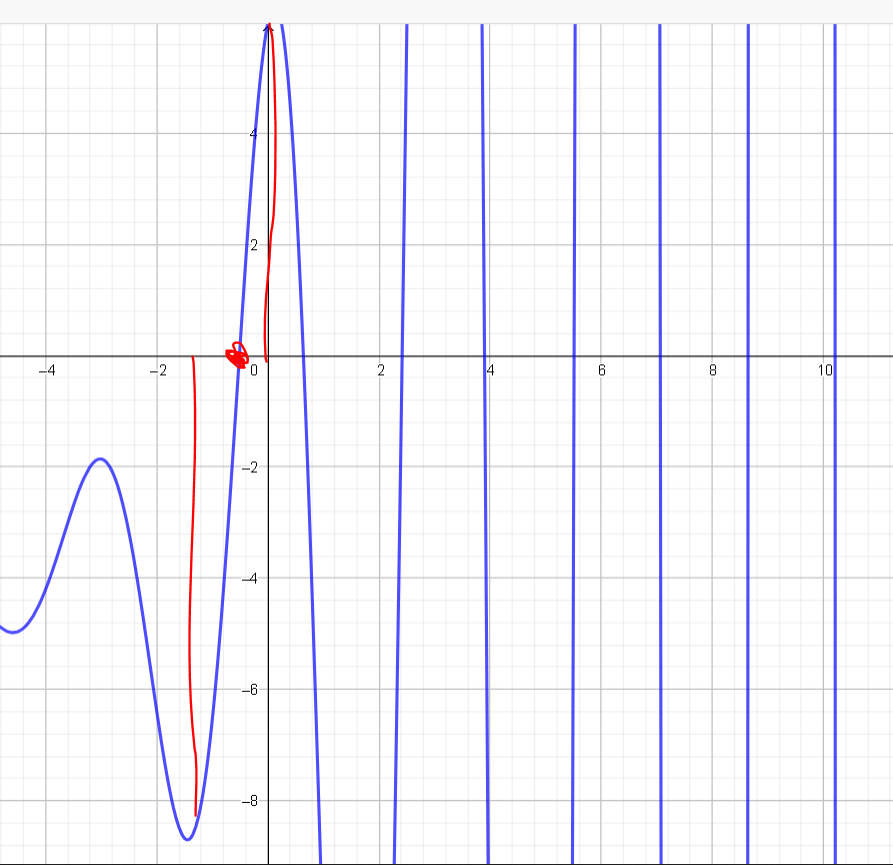
\includegraphics[width=0.6\textwidth]{f3.PNG}
    \end{figure}

    Se decidió usar 
    el Método de la Secante, la razón es que su derivada es más dificil 
    de hallar.
    Como se ve en la gráfica el punto de esa raíz es aproximadamente -0.51.
    \begin{figure}[h]
        \centering
        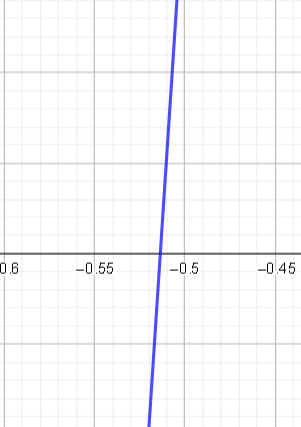
\includegraphics[width=0.2\textwidth]{f3_2.PNG}
    \end{figure}


\begin{lstlisting}
#Funcion f(x)
def f(x):
    fx = lambda x: 10*m.e**(x/2)*m.cos(2*x)-4
    return fx(x)
#no es necesario la derivada

if __name__ == "__main__":
    #nuestros dos puntos en donde se buscara la raiz
    mystr = secanteMethod([-1,0.1])
    print(mystr)#contiene todos las iteraciones
\end{lstlisting}
    El resultado de las iteraciones es:
    \begin{figure}[h]
        \centering
        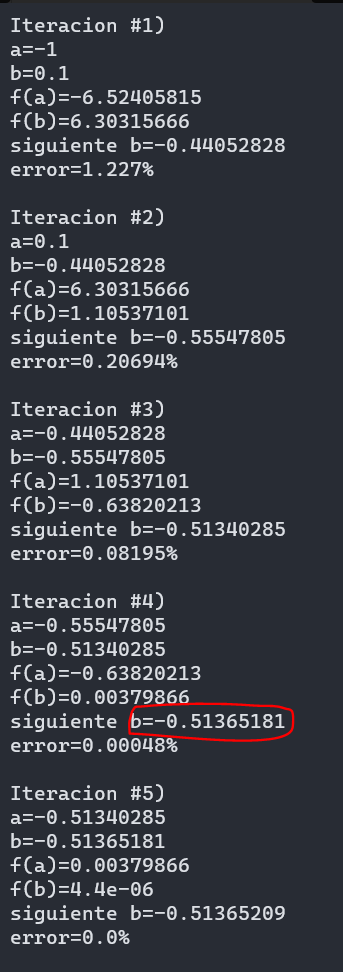
\includegraphics[width=0.3\textwidth]{f3console.PNG}
    \end{figure}
    \newpage
    \section{Problema 4}
    Calcule:
    \begin{equation}
        y =  x^2 - 2        
    \end{equation}
    
    La gráfica de la función es:
    \begin{figure}[h]
        \centering
        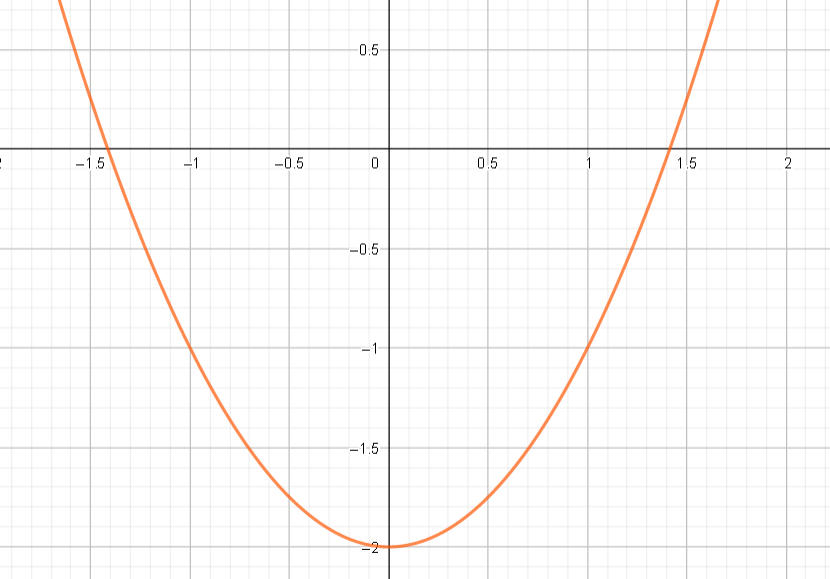
\includegraphics[width=0.6\textwidth]{f4.PNG}
    \end{figure}

    Se decidió usar 
    el Método de Newton Rapson, la razón es que su derivada es fácil 
    de hallar y por lo tanto
    podemos hallar las raíces por este método.

    Pero si suponemos que vamos a usar el punto 2, podemos ver que terminara en 
    que la solución es está cerca de 1.5, de acuerdo al Método Newton Raphson.


\begin{lstlisting}
#Funcion f(x)
def f(x):
    fx = lambda x: x**2
    return fx(x)
#Derivada de la funcion f(x)
def df(x):
    dfx = lambda x: 2*x
    return dfx(x)

if __name__ == "__main__":
    mystr = newtonRaphson(8)
    print(mystr) #contiene todos las iteraciones
\end{lstlisting}
\newpage    
El resultado de las iteraciones es:
    \begin{figure}[h]
        \centering
        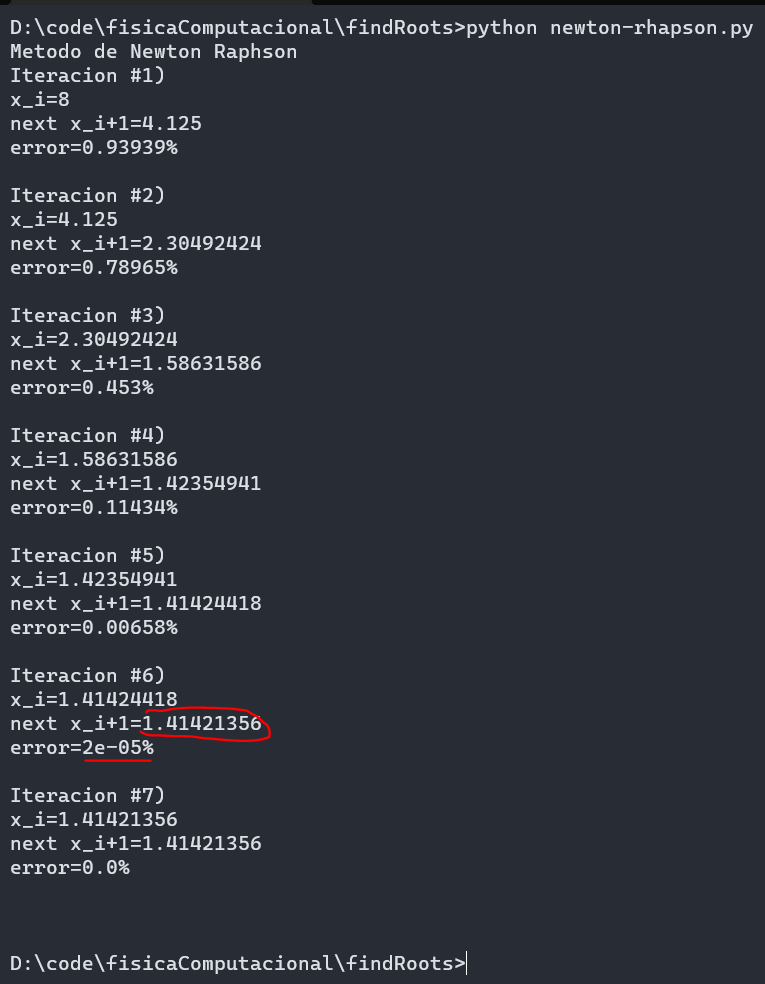
\includegraphics[width=0.4\textwidth]{f4console.PNG}
    \end{figure}

Lo que nos da un resultado aproximado de 1.41.
    \newpage
    \section{Problema 5}
    Calcule:
    \begin{equation}
        y = x^3 - 2
    \end{equation}
    La gráfica de la función es:
    \begin{figure}[h]
        \centering
        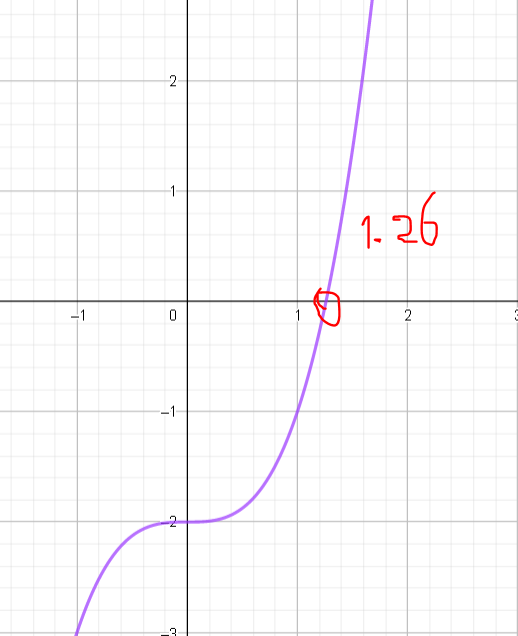
\includegraphics[width=0.4\textwidth]{f5.PNG}
    \end{figure}

    Se decidió usar 
    el Método de Newton Raphson, la razón es que su derivada es fácil 
    de hallar y por lo tanto
    podemos hallar las raíces por este método.

    Pero si suponemos que vamos a usar el punto 2, podemos ver que terminara en 
    que la solución es 1.26, de acuerdo al Método Newton Raphson.


\begin{lstlisting}
#Funcion f(x)
def f(x):
    fx = lambda x: x**3-2
    return fx(x)
#Derivada de la funcion f(x)
def df(x):
    dfx = lambda x: 3*x**2
    return dfx(x)

if __name__ == "__main__":
    mystr = newtonRaphson(3)
    print(mystr) #contiene todas las iteraciones
\end{lstlisting}
El resultado de las iteraciones es:
\newpage
    \begin{figure}[t]
        \centering
        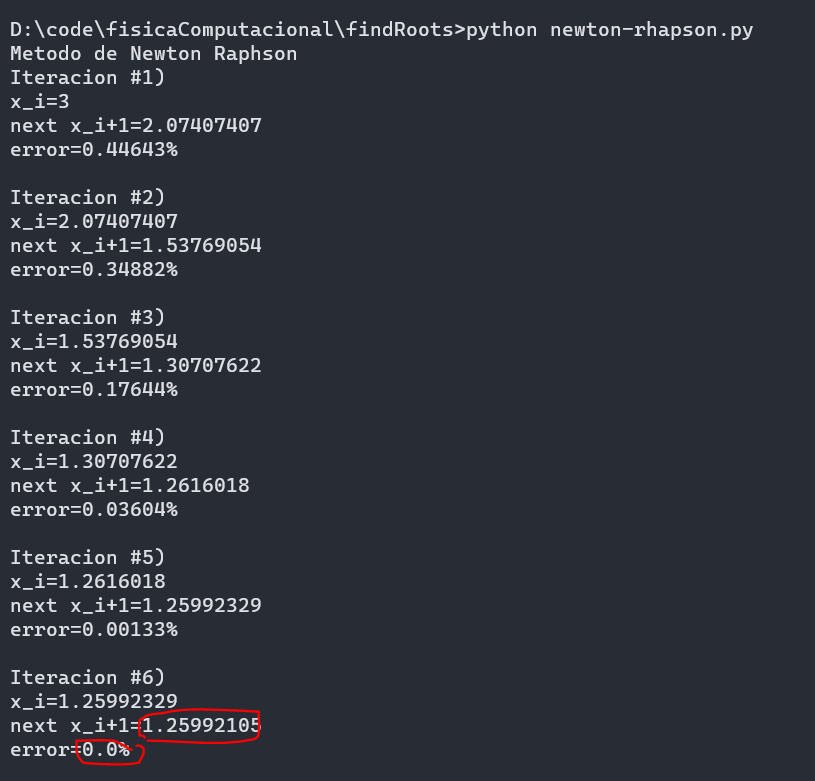
\includegraphics[width=0.6\textwidth]{f5console.PNG}
    \end{figure}

Lo que nos da un resultado aproximado de 1.2599.

    \section{Problema 6***}
    Calcule:
    \begin{equation}
        y = xcosy + ysen(x) - 2
    \end{equation}
    \newpage
    \section{Problema 7}
    Calcule:
    \begin{equation}
        y = x^3 + 4x^2 - 10
    \end{equation}

    La gráfica de la función es:
    \begin{figure}[h]
        \centering
        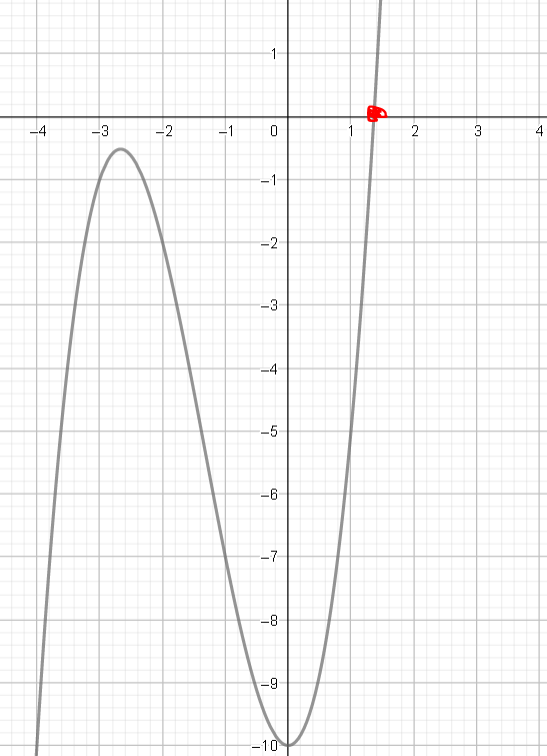
\includegraphics[width=0.4\textwidth]{f7.PNG}
    \end{figure}

    Se decidió usar 
    el Método de Newton Raphson, la razón es que su derivada es fácil 
    de hallar y por lo tanto
    podemos hallar las raíces por este método.

    Pero si suponemos que vamos a usar el punto 2, podemos ver que terminara en 
    que la solución es 1.36, de acuerdo al Método Newton Raphson.

    \begin{figure}[h]
        \centering
        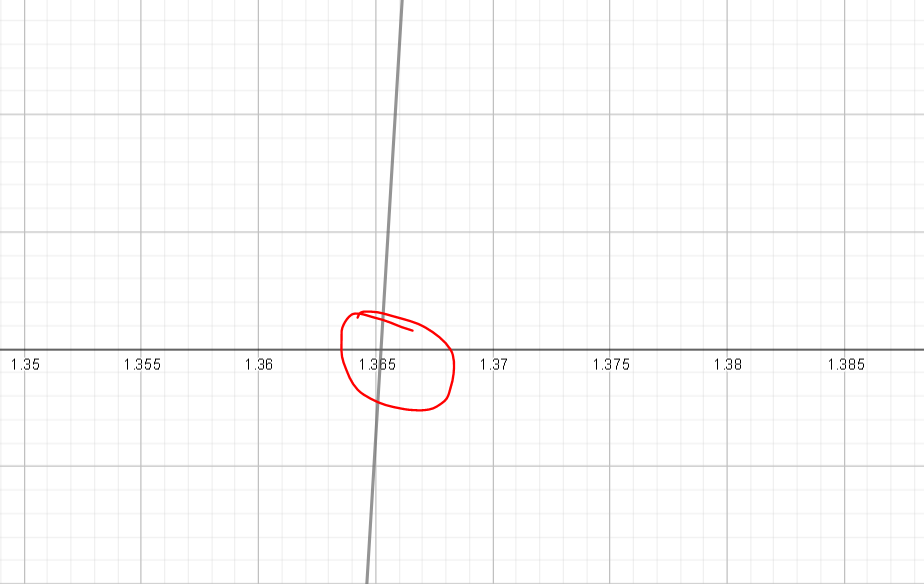
\includegraphics[width=0.5\textwidth]{f7_2.PNG}
    \end{figure}
\newpage

Las funciones iniciales son \eq{f'(x)} y \eq{f(x)}:

\begin{lstlisting}
#Funcion f(x)
def f(x):
    fx = lambda x: x**3 +4*x**2 -10
    return fx(x)
#Derivada de la funcion f(x)
def df(x):
    dfx = lambda x: 3*x**2 + 8*x
    return dfx(x)

if __name__ == "__main__":
    mystr = newtonRaphson(2)
    print(mystr) #contiene todas las iteraciones
\end{lstlisting}
    El resultado de las iteraciones es:
    \begin{figure}[h]
        \centering
        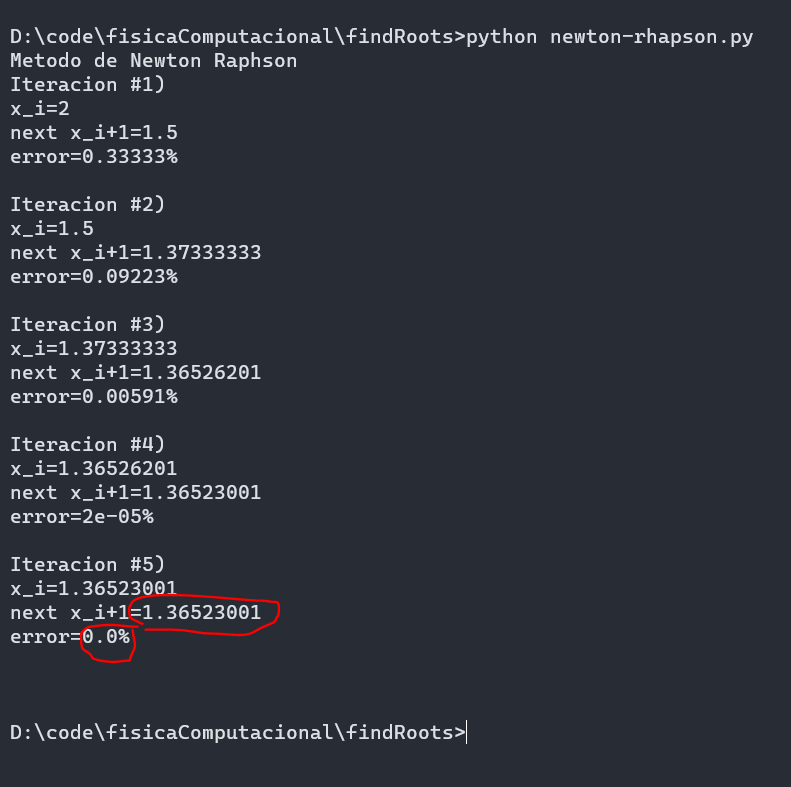
\includegraphics[width=0.6\textwidth]{f7console.PNG}
    \end{figure}

    Lo que nos da un resultado aproximado de 1.36523001.

    \clearpage
\end{document}